\documentclass{article}
\usepackage{spconf,amsmath,amssymb,graphicx,hyperref}
\usepackage{booktabs}
\usepackage{enumitem}
\usepackage{stfloats}
\usepackage{tikz}
\usetikzlibrary{arrows.meta, positioning}

% Allow long URLs to break between letters, not just at punctuation,
% so the repository link does not overflow the column.
\makeatletter
\g@addto@macro\UrlBreaks{\do\a\do\b\do\c\do\d\do\e\do\f\do\g\do\h\do\i\do\j\do\k\do\l\do\m\do\n\do\o\do\p\do\q\do\r\do\s\do\t\do\u\do\v\do\w\do\x\do\y\do\z}
\makeatother
\setcounter{topnumber}{2}
\tolerance=1200
\emergencystretch=1em

\def\x{{\mathbf x}}
\def\L{{\cal L}}

\title{Learning Chess Without Chess Knowledge: Supervised Bootstrapping
and Gated Self-Play Reinforcement Learning}

\name{Gaurav Vyas (Roll Number: 23035010370)}

\address{
Internship / Term Project Report\\
Trimester 9, Project 3\\[0.5em]
B.Sc. (Honours) Data Science and Artificial Intelligence\\
Indian Institute of Technology Guwahati, India\\
\texttt{g.vyas@op.iitg.ac.in}
}

\begin{document}
\ninept
\maketitle

\begin{abstract}
This report documents a project on training a compact neural network to play
chess without hand-coded chess knowledge, using the AlphaZero recipe: a
residual policy--value network trained first by supervised imitation of human
games and then improved by self-play guided by Monte Carlo Tree Search. A
760\,717-parameter network was trained on 676\,648 positions mined
from the Lichess open database, reaching a policy cross-entropy of
2.06. The central finding is methodological rather than architectural.
The evaluation procedure originally used scored games from White's
perspective while the network alternated colours, which rendered 159
logged evaluation points across two training runs statistically vacuous.
Once corrected scoring was applied, direct head-to-head play revealed that
300 iterations of self-play had made the model \emph{weaker} than its
own starting point ($2.5$ to $5.5$ over eight games) even as training loss
fell monotonically. Two root causes were identified and fixed: policy
targets formed from 40-visit search histograms are dominated by
sampling noise, and a mirror data-augmentation step was generating
physically impossible board states. A corrected pipeline adds acceptance gating: over 199 further
iterations the gated model measured 46.2\% against its frozen starting point
(95\% CI 37.4--55.1, indistinguishable) while the candidate stream it was
trained from averaged 42.2\% ($p=0.004$). Gating prevented the regression
without producing improvement; the residual barrier is sample efficiency.
\end{abstract}

\begin{keywords}
Reinforcement Learning, Monte Carlo Tree Search, Deep Learning,
Self-Play, Evaluation Methodology, Experimental Design
\end{keywords}

%======================================================================
\section{Introduction}
%======================================================================

Game playing has long served as a testbed for machine learning because the
reward is unambiguous and data can be generated without human annotation.
AlphaZero~\cite{silver2018alphazero} showed that a single neural network,
trained purely by self-play and guided by Monte Carlo Tree Search (MCTS),
can reach superhuman strength in chess, shogi and Go without any
domain-specific heuristics. The recipe is attractive from a data-science
standpoint because it is a closed loop: the model generates its own training
distribution, and improvements compound.

That closed loop is also its central risk. When a model manufactures
its own labels there is no held-out set whose labels are known to be correct,
and the quantity one cares about --- playing strength --- is not the quantity
being minimised. The two can move in opposite directions with no warning in
the loss curve.

This project reproduces the AlphaZero recipe at a scale that fits on a single
desktop machine, and then subjects it to the measurement discipline that
self-play demands. Section~\ref{sec:problem} states the problem and
objectives. Section~\ref{sec:method} describes the data pipeline, the
representation, the network and the two training stages.
Section~\ref{sec:results} presents the experimental results, including a
defect in the evaluation methodology that invalidated an entire training run.
Section~\ref{sec:discussion} interprets these findings, and
Section~\ref{sec:conclusion} concludes.

%======================================================================
\section{Problem Statement and Objectives}
\label{sec:problem}
%======================================================================

\subsection{Problem Statement}
Given only the rules of chess and a corpus of human games, train a neural
network with fewer than one million parameters to select strong moves,
subject to the constraint that all data generation, training and evaluation
run on a single consumer machine (six CPU cores, one mid-range GPU) within a
few hours per experiment. The network receives no evaluation function, no
opening book, no endgame tablebase and no hand-engineered features; it must
learn the value of a position and the plausibility of a move entirely from
data.

The scale constraint is not incidental. AlphaZero used 5000 TPUs and
800 simulations per move. The question here is therefore not whether the
recipe reaches grandmaster strength, but \emph{which parts of it survive
aggressive downscaling} --- and how one would know.

\subsection{Objectives}
\begin{enumerate}[noitemsep]
  \item To design and implement an end-to-end pipeline: data acquisition,
        board representation, network, search, training and evaluation.
  \item To bootstrap the network by supervised imitation of human play, and
        quantify the resulting move-prediction quality.
  \item To improve the bootstrapped network by self-play reinforcement
        learning, and \emph{verify} that improvement with a metric valid
        under self-play conditions.
  \item To diagnose any failure to improve, and to make the training
        procedure robust against it.
\end{enumerate}

Objective~3 is deliberately phrased to separate \emph{running} the algorithm
from \emph{demonstrating} that it worked. That separation turned out to carry
the entire result.

%======================================================================
\section{Methodology}
\label{sec:method}
%======================================================================

\subsection{Overall Workflow}

\begin{figure}[t]
\centering
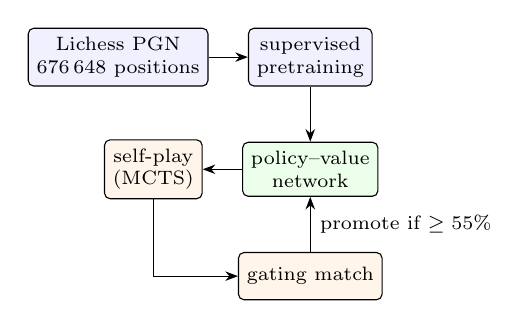
\begin{tikzpicture}[
  node distance=5mm,
  box/.style={draw, rounded corners=2pt, align=center, font=\scriptsize,
              minimum height=6mm, inner xsep=3pt},
  >={Stealth[length=1.6mm]}]
\node[box, fill=blue!6] (pgn) {Lichess PGN\\ 676\,648 positions};
\node[box, fill=blue!6, right=of pgn] (sup) {supervised\\ pretraining};
\node[box, fill=green!8, below=7mm of sup] (net) {policy--value\\ network};
\node[box, fill=orange!8, left=of net] (sp) {self-play\\ (MCTS)};
\node[box, fill=orange!8, below=7mm of net] (gate) {gating match};
\draw[->] (pgn) -- (sup);
\draw[->] (sup) -- (net);
\draw[->] (net) -- (sp);
\draw[->] (sp) |- (gate);
\draw[->] (gate) -- node[right, font=\scriptsize] {promote if $\geq 55\%$} (net);
\end{tikzpicture}
\caption{The two-stage pipeline. Supervised pretraining supplies the initial
policy; self-play then proposes updates, which are accepted only if they win
a head-to-head match against the incumbent weights.}
\label{fig:pipeline}
\end{figure}

Training proceeds in two stages (Figure~\ref{fig:pipeline}). Stage~1 fits the
network to human moves, giving it an immediate grasp of openings and basic
tactics. Stage~2 replaces the human teacher with the network's own search. An
acceptance gate, added after the diagnosis in Section~\ref{sec:regression},
sits between the two.

\subsection{Data Pipeline}

Data come from the Lichess open database~\cite{lichess}, distributed as
Zstandard-compressed PGN. Monthly dumps are streamed and decompressed
incrementally rather than materialised, since a single month exceeds
available memory when expanded.

Quality filtering is applied at the game level: only games in which
\emph{both} players are rated at least 1750 Elo are retained. This admits
roughly 12\% of games, giving a corpus of 676\,648 positions from about
9600 games out of the 80\,000 read.

Each retained position yields one training example: an $18\times8\times8$
tensor, the index of the move the human actually played, and the game outcome
expressed from the side to move. A subset of 40\,000 examples is frozen
as a \emph{rehearsal anchor} (Section~\ref{sec:selfplay}), and 6000
positions taken five to eight plies into games are retained as a self-play
opening curriculum.

\subsection{Representation and Action Encoding}
\label{sec:repr}

The board is encoded as 18 binary planes of $8\times8$: twelve
piece-placement planes (six piece types $\times$ two colours), four
castling-rights planes, one en-passant plane and one side-to-move plane.

The action space follows the Leela Chess Zero scheme~\cite{lczero}: each of
the 64 origin squares carries 73 move planes --- 56
queen-style moves (eight directions $\times$ seven distances), eight knight
moves and nine underpromotions --- giving $64\times73=4672$ actions, indexed
as $\text{index} = \text{from} \times 73 + \text{plane}$. A round-trip
self-test verifies that every legal move in a sample of positions encodes and
decodes without collision.

\subsection{Network Architecture}

The network is a residual convolutional trunk~\cite{he2016resnet} with two heads: a $3\times3$
convolution mapping 18 input planes to 64 channels, ten residual
blocks of two $3\times3$ convolutions with batch normalisation~\cite{ioffe2015batchnorm}, a policy head
($1\times1$ convolution to 73 planes, reshaped to 4672 logits)
and a value head ($1\times1$ convolution to one channel, a fully connected
layer to 64 units, and a scalar through $\tanh$). Total trainable
parameters: 760\,717.

The heads share the trunk, so a single representation must serve both
\emph{who is winning} and \emph{which moves are plausible}.

\subsection{Stage 1: Supervised Pretraining}

Given a position $s$, the human move $m$ and the outcome $z\in\{-1,0,+1\}$,
the loss is
\begin{equation}
\L_{\text{sup}} = -\log p_{\theta}(m \mid s) + \big(v_{\theta}(s)-z\big)^2 ,
\end{equation}
optimised with Adam~\cite{kingma2015adam}, a cosine learning-rate schedule from $10^{-3}$ to
$10^{-4}$, and batch size 256 for three epochs.

\subsection{Stage 2: Self-Play Reinforcement Learning}
\label{sec:selfplay}

The network plays itself. Each move is selected by MCTS~\cite{kocsis2006uct, browne2012mcts}, which descends the
tree by the PUCT rule~\cite{rosin2011puct}
\begin{equation}
U(s,a) = Q(s,a) + c_{\text{puct}}\,P(s,a)\,\frac{\sqrt{N(s)}}{1+N(s,a)},
\end{equation}
where $Q$ is the child's mean value, $P$ the network prior and $N$ the
visit count. Leaves are evaluated by the network, terminal positions by the
true result, and Dirichlet noise is added at the root during self-play only.
The normalised visit distribution $\pi$ becomes the policy target and the
result $z$ the value target, giving the AlphaZero loss
\begin{equation}
\L = \mathbb{E}_{s}\Big[-\pi^{\top}\log p_{\theta}(s)
      + \big(v_{\theta}(s)-z\big)^2\Big] + \lambda\lVert\theta\rVert^2 .
\label{eq:azloss}
\end{equation}

Two additions guard against catastrophic
forgetting~\cite{mccloskey1989catastrophic}, the first being rehearsal on a
frozen exemplar set~\cite{rebuffi2017icarl}: 30\% of every minibatch comes
from the anchor, and self-play games start from curriculum positions 85\% of
the time. Self-play runs in six CPU workers overlapped with GPU training, so
self-play weights lag one iteration --- a standard relaxation.

\subsection{Evaluation Methodology}
\label{sec:evalmethod}

Because self-play provides no held-out labels, playing strength must be
measured by playing games. Three properties are required for such a
measurement to carry information:

\begin{enumerate}[noitemsep]
  \item \textbf{Correct attribution.} Score from the \emph{network's}
        perspective: if it alternates colours and results are tallied as raw
        PGN strings, every win as Black counts as a loss.
  \item \textbf{Independent games.} Two deterministic players replay one
        identical game, so an $N$-game match carries one game of information
        unless openings are randomised.
  \item \textbf{An informative opponent.} A frozen reference measures
        progress; one that improves alongside the model measures nothing.
\end{enumerate}

All three were violated originally; their restoration is what makes
Section~\ref{sec:results} interpretable.

%======================================================================
\section{Experiments and Results}
\label{sec:results}
%======================================================================

\subsection{Experimental Setup}
All experiments ran on an Intel i5-12400F (6C/12T) with an NVIDIA RTX
3060, in PyTorch~2.13~\cite{paszke2019pytorch} with
\texttt{python-chess}~\cite{pythonchess}. Self-play is CPU-bound, the GPU
serving only batched gradient steps, so low GPU utilisation is expected.
Throughput at twelve games per iteration on six workers is 42\,s at 40
simulations, 180\,s at 128.

\subsection{Supervised Pretraining}
Policy cross-entropy fell from 3.90 to 2.06 over three epochs
(Figure~\ref{fig:pretrain}) --- roughly 13\% probability on the move a strong
human actually chose, against a uniform-over-legal-moves baseline near 3.4.

\begin{figure}[t]
\centering
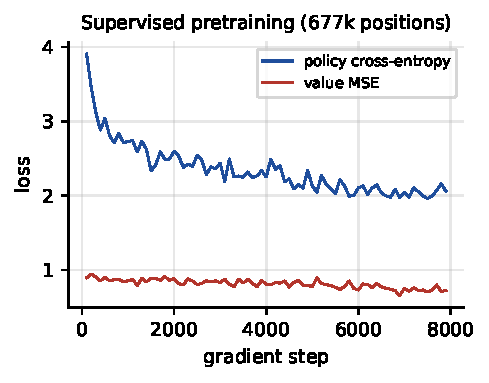
\includegraphics[width=0.70\linewidth]{figures/pretrain_loss.pdf}
\caption{Supervised stage. Policy cross-entropy converges to $\approx 2.06$;
value MSE plateaus near 0.73, reflecting the intrinsic difficulty of
predicting a game outcome from a single mid-game position.}
\label{fig:pretrain}
\end{figure}

Behavioural probes confirm this reflects real competence: the raw policy
assigns 0.594 to \texttt{e4} and 0.313 to \texttt{d4}, answers \texttt{e4}
with \texttt{e5} or \texttt{c5}, captures a hanging queen and finds mate in
one, scoring 85\% against a random opponent.

\subsection{A Defect in the Evaluation Metric}
\label{sec:metric}

The evaluation harness alternated the network between colours but scored
wins-as-White plus half the draws. Combined with the absence of opening
randomisation, the consequence is a tally that can only be symmetric, and a
score pinned near 50\% regardless of the model:

\begin{center}\ttfamily\scriptsize
[iter 454] eval: \{1-0: 0, 0-1: 0, 1/2-1/2: 10\} (score 50\%)\\{}
[iter 499] eval: \{1-0: 0, 0-1: 0, 1/2-1/2: 10\} (score 50\%)
\end{center}

159 evaluation points across two runs conveyed no information. The same
defect reported the pretrained model at 44\% against a random opponent
when its true score is 85\%.

\subsection{Self-Play Regressed}
\label{sec:regression}

With corrected scoring and randomised openings, the final model of the
300-iteration self-play run was played directly against its own
starting point over eight games:
\begin{center}
\textbf{v5 \texttt{iter\_500} \quad 2.5 -- 5.5 \quad pretrained
\texttt{iter\_200}}
\end{center}
Self-play made the model \emph{worse}. Throughout those 300 iterations
the training loss fell monotonically from 2.36 to 1.85
(Figure~\ref{fig:v5}). Loss is not a strength signal.

\begin{figure}[t]
\centering
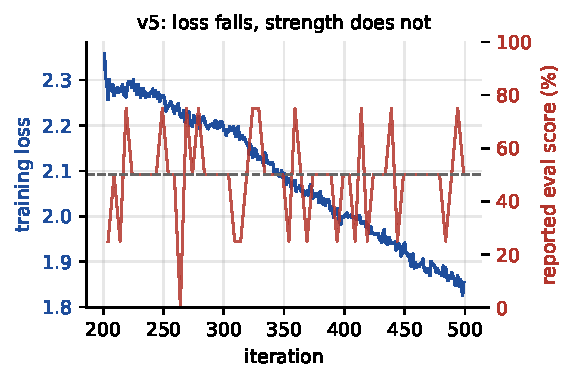
\includegraphics[width=0.70\linewidth]{figures/v5_regression.pdf}
\caption{The v5 run. Training loss (left axis) falls throughout, while the
reported evaluation score (right axis) is pinned at 50\% by the defect
of Section~\ref{sec:metric}. Direct head-to-head play shows the model in fact
got weaker.}
\label{fig:v5}
\end{figure}

An earlier run without the rehearsal anchor failed more visibly: its policy
degenerated to opening with \texttt{f3}, its value head returned $-0.270$ for
the balanced initial position, and it no longer captured a hanging queen ---
textbook catastrophic forgetting~\cite{mccloskey1989catastrophic}. Rehearsal prevented that collapse, but
preventing collapse is not improvement.

\subsection{Diagnosis: Search Quality Versus Target Quality}

A natural hypothesis is that search is too weak to teach the network. It was
tested by playing MCTS against the same network's raw policy head at varying
simulation counts (Figure~\ref{fig:sims}). Search wins comfortably ---
79\% at only 40 simulations --- so the hypothesis is false.

\begin{figure}[t]
\centering
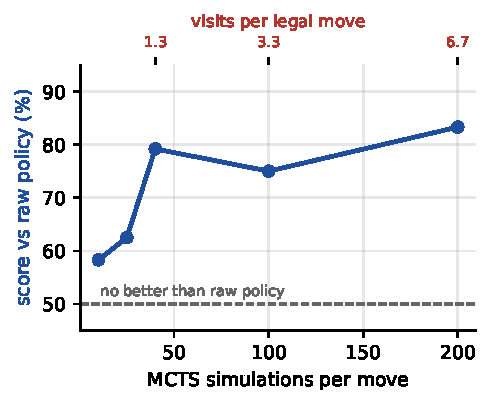
\includegraphics[width=0.70\linewidth]{figures/sims_scaling.pdf}
\caption{MCTS against the network's own greedy policy. Search is clearly
stronger than the raw policy even at 40 simulations, so the
\emph{argmax} of the search is a good move; the upper axis shows why the
\emph{distribution} is nonetheless a poor target.}
\label{fig:sims}
\end{figure}

The distinction matters. Equation~\eqref{eq:azloss} trains on the full visit
distribution $\pi$, not on its argmax. With 40 simulations spread over
roughly 30 legal moves, $\pi$ is a histogram of about 1.3 visits
per move: its mode is informative, its shape is sampling noise. Fitting a
sharp supervised policy to that noise flattens it.

A second, independent defect compounded this. A mirror augmentation flipped
board files on half of every minibatch but did not exchange the kingside and
queenside castling planes. After a file flip the king stands on \texttt{d1}
while the kingside-castling plane remains set --- a position that cannot
arise in chess, paired with features contradicting the pieces. Chess is not
mirror-symmetric, precisely because castling and pawn direction break the
symmetry; roughly half of every batch, including the rehearsal slice, was
corrupted.

\subsection{Corrected Pipeline}

Four changes: castling-aware augmentation (positions retaining castling
rights are not mirrored), 128 simulations instead of 40 ($\approx4.3$ visits
per legal move), 80 gradient steps instead of 200, and a lower learning
rate.

The decisive change is \emph{acceptance
gating}~\cite{silver2017alphagozero}: self-play always generates from the
best weights so far, and updated weights reach the deployed model only after
scoring at least 55\% against the incumbent.

\begin{figure}[t]
\centering
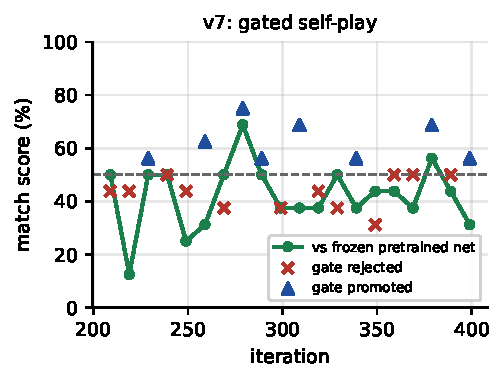
\includegraphics[width=0.70\linewidth]{figures/v7_progress.pdf}
\caption{The corrected run. Each gate point plots the candidate's score
against the incumbent (markers) and against the frozen pretrained network
(line). The dashed line is equal strength.}
\label{fig:v7}
\end{figure}

The run completed 199 iterations, settled by a 40-game match (random
openings, alternating colours) against the frozen network; at 40 games the
standard error is 7.9 points, against 17.7 for the eight-game training
matches (Table~\ref{tab:v7}).

It scored 46.2\% (95\% CI 37.4--55.1, $z=-0.83$): no detectable
difference from its starting point, with both models beating a random mover
identically (86.2\% and 87.5\%). Self-play produced no improvement --- but
nor the regression of Section~\ref{sec:regression}.

The mechanism is visible in the intermediate data: the \emph{candidate}
network, trained continuously and repeatedly rejected, averaged 42.2\% over
20 measurements ($z=-2.87$, $p=0.004$). Self-play was still degrading the
network, and the gate kept that damage out of the deployed weights.

The guarantee is weaker than it appears, however: 8 of 20 gates promoted
against 7.8 expected under the null of no improvement
(Section~\ref{sec:discussion}).

\begin{table}[t]
\centering
\caption{Corrected run. Head-to-head figures are 40-game matches with
randomised openings; intervals are 95\% CIs. Training loss fell
2.560$\rightarrow$2.473 over 199 iterations.}
\label{tab:v7}
\begin{tabular}{lr}
\toprule
Quantity & Value \\
\midrule
Gate promotions (noise predicts 7.8) & 8 / 20 \\
Candidate vs.\ baseline (20 gates)   & 42.2\% ($p=0.004$) \\
\textbf{Gated model vs.\ baseline}   & \textbf{46.2\%} [37.4, 55.1] \\
Gated model vs.\ random             & 86.2\% [79.2, 93.3] \\
Baseline vs.\ random                & 87.5\% [80.7, 94.3] \\
\bottomrule
\end{tabular}
\end{table}

%======================================================================
\section{Discussion}
\label{sec:discussion}
%======================================================================

\noindent\textbf{Optimisation success is not task success.}
A falling loss curve coexisted with a model getting worse at the task.
Equation~\eqref{eq:azloss} is computed against targets the model itself
produced, so minimising it measures self-agreement, not chess strength. Every
self-training pipeline shares this structure and this failure mode.

\noindent\textbf{A broken metric is worse than no metric.}
The defect was costly not because it was subtle but because it was
\emph{reassuring}: it returned 50\%, a plausible constant, for 159
consecutive measurements across two multi-hour runs. The symmetric tallies
were visible in every log line and read as evenly matched play rather than as
the signature of a bug.

\noindent\textbf{Sample efficiency governs downscaling.}
The failure was not a shortage of compute but its allocation: cutting
simulations from 800 to 40 preserves the argmax while destroying the
calibration of the distribution, and Equation~\eqref{eq:azloss} consumes the
distribution. When downscaling, the question is not what a parameter does at
full scale but which statistic of it the loss actually reads.

\noindent\textbf{A safeguard is only as good as its test.}
Gating worked in aggregate --- rejected candidates were significantly worse
than baseline, the protected model was not --- but individual decisions were
indistinguishable from chance, an eight-game match resolving nothing at this
effect size. Having diagnosed one metric that measured nothing, we built a
safeguard and assumed it worked: the same error one level up.

\noindent\textbf{Limitations.}
The value head plateaus at MSE 0.73, and absolute strength is not calibrated
against a rated engine, so all results are relative comparisons.

%======================================================================
\section{Conclusion and Future Work}
\label{sec:conclusion}
%======================================================================

Supervised pretraining on 676\,648 Elo-filtered Lichess positions gave a
760\,717-parameter network that plays principled openings, wins material and
finds simple mates, scoring 85\% against a random opponent.

The substantive contribution is negative and methodological. Self-play
as originally implemented degraded the model, and the evaluation procedure
could not detect it. Correcting the metric exposed the regression; controlled
experiments isolated one statistical cause (visit histograms too sparse to be
distributional targets) and one representational cause (an augmentation
producing illegal boards); and gating held the deployed model level (46.2\%,
CI 37.4--55.1) while rejected candidates drifted significantly below
baseline. Self-play at this scale neither helped nor, once gated, hurt. The
binding constraint is sample efficiency: 128 simulations give 4.3 visits per
legal move against roughly 27 for AlphaZero.

Future work follows from the diagnosis: batched leaf evaluation and
subtree reuse would raise simulations several-fold at equal wall-clock cost;
sequential-probability-ratio testing~\cite{wald1945sprt} would set gate
decisions at a stated confidence level; and calibration against Stockfish at
reduced strength would yield an Elo estimate~\cite{elo1978rating}.

%======================================================================
\section{Artifacts and Demonstrations}
%======================================================================

\begin{itemize}[noitemsep]
  \item \textbf{Code:} \url{https://github.com/realgauravvyas/chess-ai}
        --- network, search, both training stages, dashboard, and the
        \texttt{experiments/} scripts reproducing every number here.
        \texttt{RESULTS.md} records the findings and defects fixed.
  \item \textbf{Dashboard:} \texttt{dashboard/server.py} --- play any
        checkpoint, inspect the principal variation, watch training live.
  \item \textbf{Video:} \textsc{[URL to be added]}
\end{itemize}

\noindent
Presentation follows standard guidance~\cite{gopen1990science}.
AI-assisted tools aided code review and drafting; all results are the
author's own and reproducible from the repository.

\vfill\pagebreak
{\fontsize{8}{9}\selectfont
\bibliographystyle{IEEEbib}
\bibliography{refs}
}

\end{document}
